\section{Electronics Design}
\label{sec:hardware}

This section describes the of the electronics of the SM4 stepper motor controller.
First, the critical components are selected and preliminary design is done based on the requirements stated in the Section~\ref{sec:requirements}.
Second, the design of the electronics is described.
There were two electronics revisions, where different stepper motor driver \acs{ic} was used in each of them and there were some also some minor changes.
In the description the second revision is prioritized with the the exception of the design of the circuit of the stepper motor controller \acs{ic} where both of the revisions are described.
Further, manufacturing of the \acs{pcb} and assembly in JLCPCB is described.

In the Figure~\ref{fig:sm4diagram}, we can see the block diagram of the controller.
The central part is the \acs{mcu}, which is connected to the two stepper motor drivers and encoders (hardware encoders are only available in the second electronics revision).
Further there are also peripheral chips and components used to utilize the \acs{can}, I\textsuperscript{2}C and \acs{usb} buses.
The whole controller is powered by the power system providing correct voltages and electrical protection.

\begin{figure}[H]
    \centering
    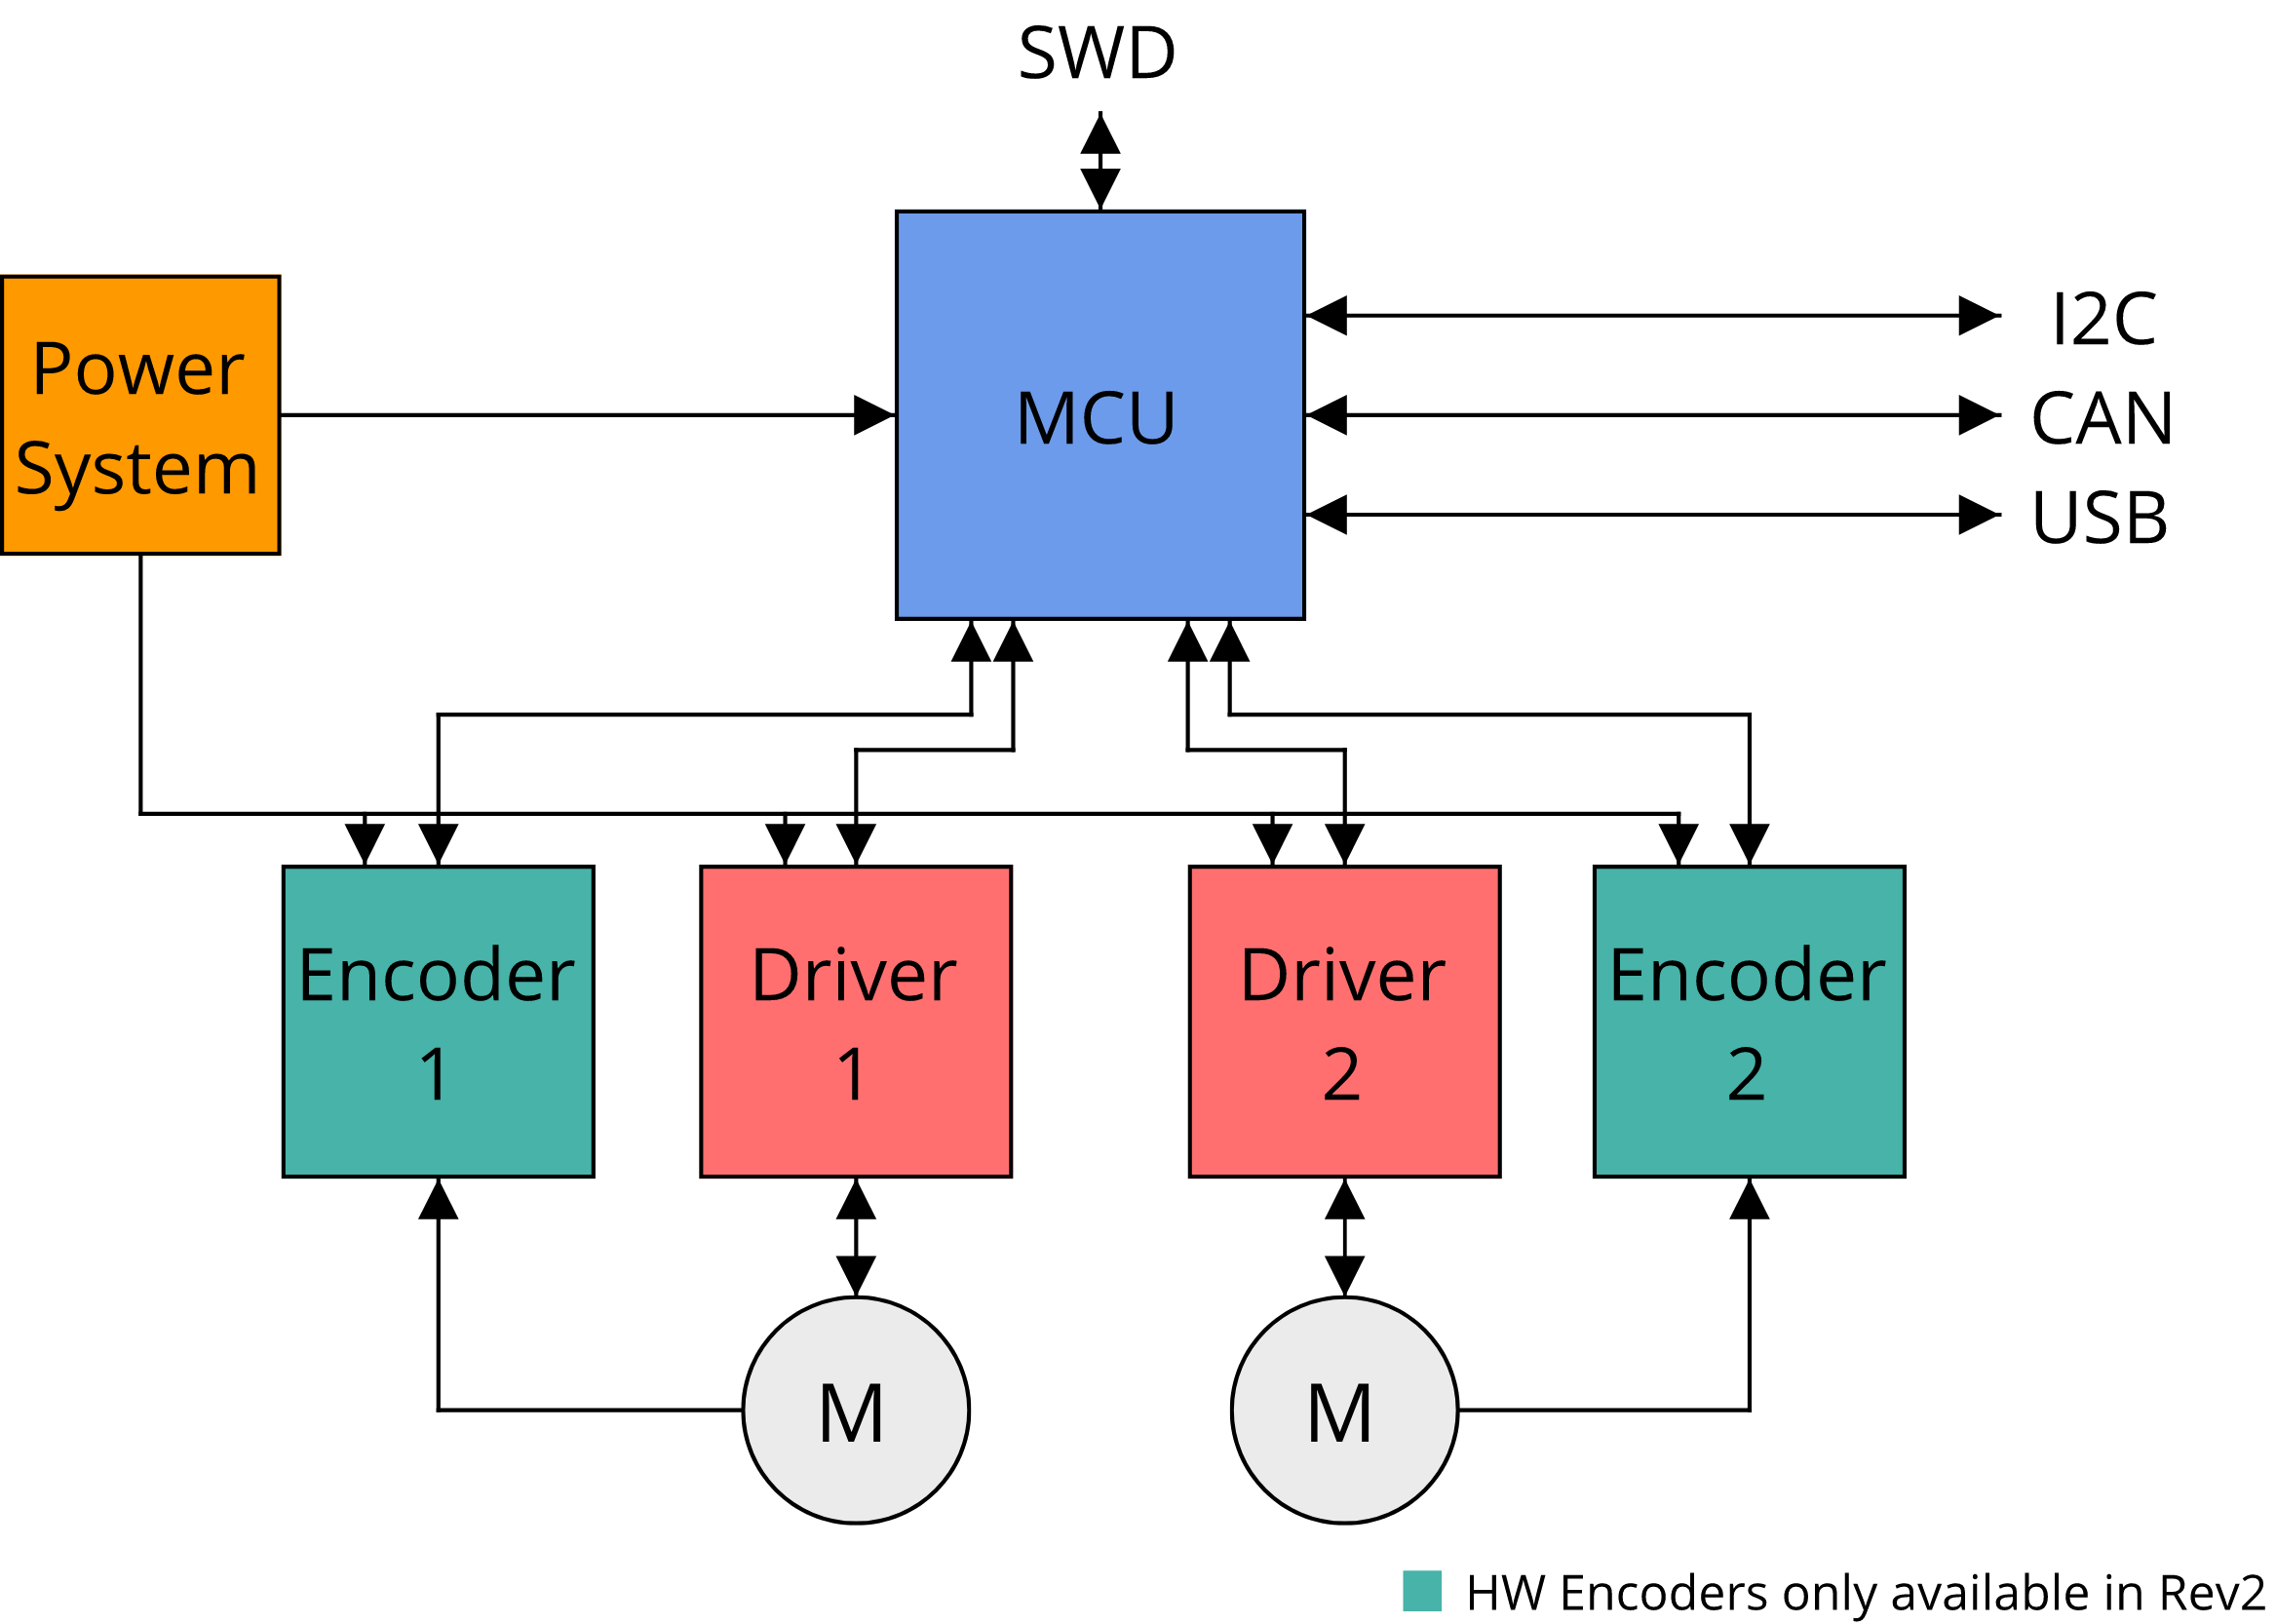
\includegraphics[width=\textwidth]{obrazky/sm4_block_diagram}
    \caption{The block diagram of the SM4 stepper motor controller.}
    \label{fig:sm4diagram}
\end{figure}


\subsection{Hardware Design Choices}
\label{subsec:hardware_design_choices}
In this section, we describe the choices made in the beginning of the design process, ones that are vital to the functionality of the whole system.
The design choices are based on the requirements stated in the Section~\ref{sec:requirements}, the related work described in the Chapter~\ref{ch:related_work} and our prior experience.

\subsubsection{MCU}
\label{subsubsec:mcu}
The most critical component of the stepper controller is the \acs{mcu}.
The MCU needs to accommodate for the outer communication interfaces as well as the internal ones.
That means that as for the outer communication interfaces, it needs to have peripherals for CAN bus, I\textsuperscript{2}C and USB, as stated in the requirement \textbf{C-03}.
The internal communication interfaces are revision dependent, however the stepper controllers generally require, GPIOs, PWM outputs, serial interfaces and for the possible future encoder support it should require incremental encoder interfaces and SPIs for SSI bitbanging (as stated in requirement \textbf{FR-08}).
As was described in the Chapter on Related work~\ref{ch:related_work}, we decided to make the move from Cortex-M0 and Cortex-M0+ based ARM MCUs to more powerful Cortex-M4 MCUs.
The biggest advantage of these cores is that they fully support atomic instructions, improving memory safety in ISRs, and also that they have FPU (Floating Point Unit).

Given the past experience with STM32 family of ARM microcontrollers, we decided to select the STM32F4 product line, more specifically with the STM32F405RGT6 which features one megabyte of flash and 192 kilobytes of RAM and can be run with the 168 MHz clock\cite{stmicro_stm32f405rg_nodate}.
The block diagram of the MCU with the core features and peripherals can be seen in the Figure~\ref{fig:stm32f405_block_diagram}.

\begin{figure}[H]
    \centering
    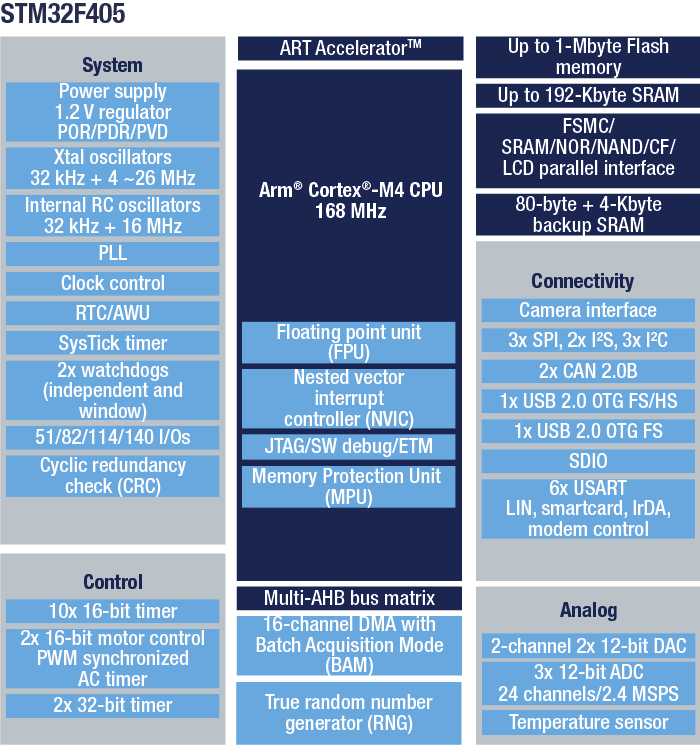
\includegraphics[width=0.7\textwidth]{obrazky/stm32f405_block_diagram}
    \caption{The block diagram of the STM32F405RG MCU~\cite{stmicro_enbd_stm32f405_1mbjpg_nodate}.}
    \label{fig:stm32f405_block_diagram}
\end{figure}

This MCU conforms to all the requirement and has enough peripherals to support future development.

\subsection{Stepper motor driver IC}
\label{subsec:stepper_ic}
In order to select a proper driver IC for the SM4 stepper motor controller a simplified comparison was performed.
Since the beginning we were aiming at using the Trinamic made stepper motor driver ICs since there are very good references from the 3D printing community\cite{prusa_original_2017,prusa_original_2019,3daddict_stepper_2020} for them, and we wanted to secure silent function of the motor controller.
With the prior experience with DRV8825 and the A4988 modules described in the Chapter on Related work~\ref{ch:related_work}, we decided to select two drivers from Trinamic - the first hardware revision utilizes the TMC2100-TA as we aimed for as simple chip as possible and also maximum voltage of about 43~V, while the second hardware revision utilizes the TMC2226-SA, which is a more modern, and a fully featured stepper motor driver \acs{ic}, which also has higher peak current.
By selecting these two stepper driver \acs{ic}s, we are conforming to the requirements \textbf{C-01} and \textbf{C-02}.
The comparison can be seen in the following table:

\begin{sidewaystable}
    \centering
    \begin{tabular}{ |p{2.5cm}|p{2cm}|p{2cm}|p{2cm}|p{2.5cm}|p{2.5cm}|p{2cm}|p{4cm}| }
        \hline
        Name & Operating Voltage & Maximum current & Control Interface & Configuration Interface & Microstepping & Package & Advanced Features \\
        \hline
        \hline
        DRV8825\cite{texas_instruments_drv8825_2014} & 8.2-45~V & max 2.5~A (properly cooled, at 24~V, 25~\textdegree) & STEP/DIR & GPIO & up to 32 & HTSSOP28 & None \\
        \hline
        A4988\cite{allegro_microsystems_a4988_2014} & max 35~V & max 2 A & STEP/DIR & GPIO & up to 16 & QFN28ET & None \\
        \hline
        TMC2100\cite{trinamic_tmc2100-datasheet_2018} & max 46~V & max 2 A (2.5 A peaks, properly cooled) & STEP/DIR & GPIO & up to 256 & TQFP48 / QFN36 & MicroPlyer\texttrademark, SpreadCycle\texttrademark, StealthChop\texttrademark \\
        \hline
        TMC2130\cite{trinamic_tmc2130-datasheet_2018} & max 46~V & max 2 A (2.5 A peaks, properly cooled) & STEP/DIR & SPI & up to 256 & TQFP48 / QFN36 & MicroPlyer, SpreadCycle\texttrademark, StealthChop\texttrademark, ChopSync\texttrademark, CoolStep\texttrademark, StallGuard\texttrademark \\
        \hline
        TMC2209\cite{trinamic_tmc2209_2019} & max 29~V & max 2 A (2.8 A peaks) & STEP/DIR & UART & up to 256 & QFN28 & MicroPlyer\texttrademark, SpreadCycle\texttrademark, StealthChop2\texttrademark, CoolStep\texttrademark, StallGuard4\texttrademark \\
        \hline
        TMC2226\cite{trinamic_tmc2226_2020} & max 29~V & max 2 A (2.8 A peaks) & STEP/DIR & UART & up to 256 & HTSSOP28 & MicroPlyer\texttrademark, SpreadCycle, StealthChop2\texttrademark, CoolStep\texttrademark, StallGuard4\texttrademark \\
        \hline
    \end{tabular}
    \caption{Comparison of stepper motor driver ICs}
    \label{tab:driver_ic_comparison}
\end{sidewaystable}
\newpage

\subsubsection{SM4 power design}
\label{subsubsec:power_design}
The power design of the SM4 stepper motor controller is fairly simple.
According to the requirements, the only requirement for it is to provide basic electrical safety features, such as fuses and reverse voltage protection \textbf{FR-07}.
The controller features two power rails - one for the power electronics, that can utilize quite high voltages and one 5~V for the MCU and the peripheral circuits.
With the first revision, we were considering using a single power-rail with all voltages derived from the power electronics one.
This was however dismissed as a buck converter from quite a high voltage would be required and designing a buck converter is out of the scope of this project and also the motor controller was never meant to be used as a standalone device, meaning that another device could provide the power for the 5~V rail.
The buck converter would also pose \acs{emi} (\acl{emi}) problems and would increase the price of the motor controller.
In the end, the 5~V power rail is properly fused, filtered and given that the voltage may come from different sources also merged using diodes.
The power electronics rail on the other hand is only filtered.
A block diagram depicting the power system can be seen in the Figure~\ref{fig:power_diagram}.

\begin{figure}[H]
    \centering
    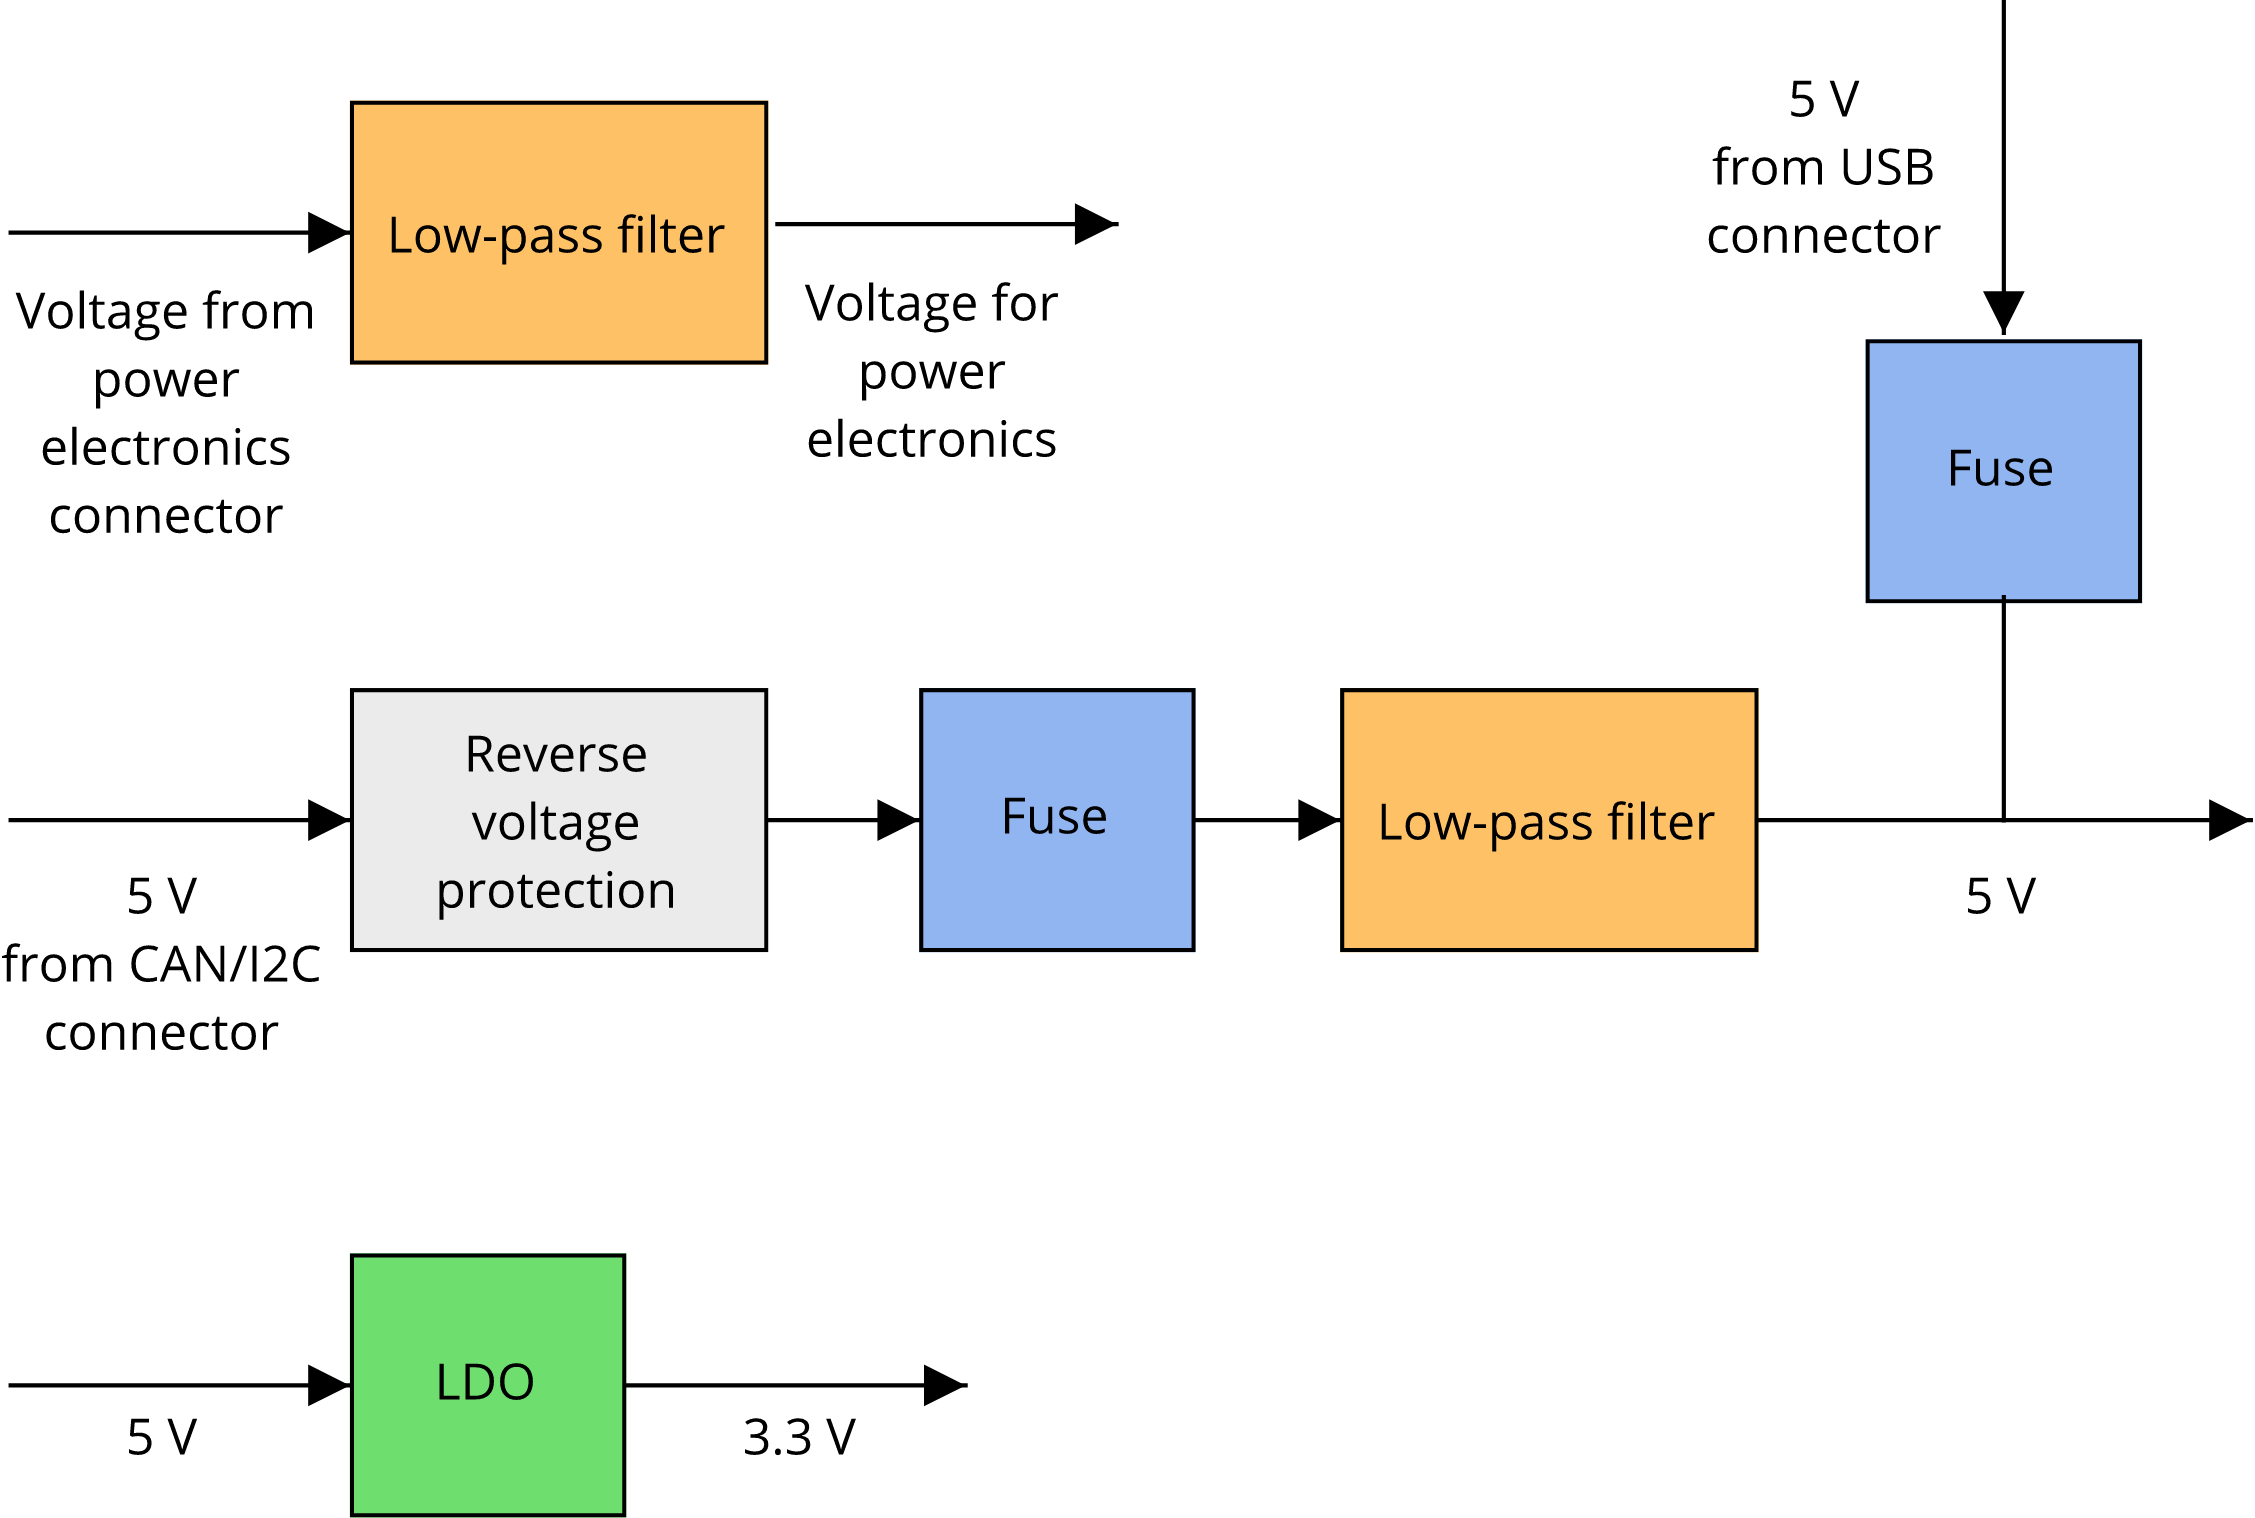
\includegraphics[width=0.9\textwidth]{obrazky/power_block_diagram}
    \caption{The block diagram of the power system.}
    \label{fig:power_diagram}
\end{figure}

\subsubsection{PCB}
\label{subsubsec:pcb_design}
In order for this project to serve as a testbed for new manufacturing technologies, the \acs{pcb} (\acl{pcb}) was designed as 4-layer.
The ability to design the board as a 4-layer one was enabled by the 4-layer \acs{pcb} manufacturing price decrease by China-based \acs{pcb} manufacturing companies.
Big advantage of designing the \acs{pcb} as 4-layer one was speedup of hardware development - the 4-layer stackup can be utilized so that there is no need to route power to the \acs{ic}s.
In our case we chose the inner layers to be filled with copper planes - one connected to \acs{gnd} and the other one connected to +3.3~V.
This way whenever a connection to +3.3V or \acs{gnd} was required, simply connecting the pad to new via close-by was sufficient.
Apart from being used for power distribution, the large copper planes allow for better \acs{pcb} cooling and also for some minor signal connections in cases routing using the outer layers would prove difficult.
The used stackup can be seen in the Figure~\ref{fig:stackup}.

\begin{figure}[H]
    \centering
    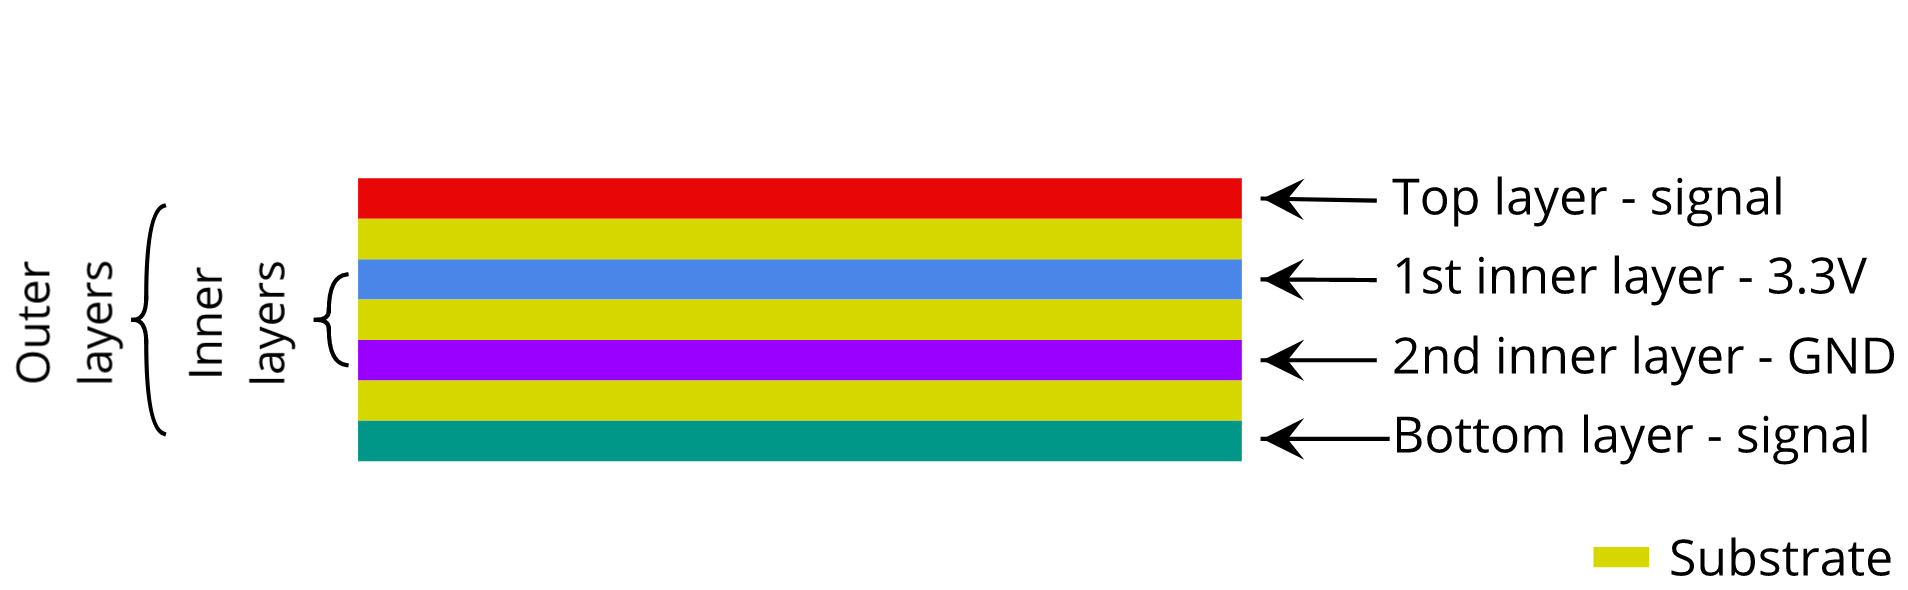
\includegraphics[width=0.9\textwidth]{obrazky/stackup}
    \caption{The 4-layer PCB stackup.}
    \label{fig:stackup}
\end{figure}

Another way to test manufacturing capabilities was utilizing the automated assembly service provided by the China-based PCB manufacturers.
This not-only saved a lot of time with manual assembly, but also enabled us to use smaller components than before - the imperial size 0402.

As for testing out EDA (Electronic Design Aid) software, the KiCAD EDA was used instead of the well-known Eagle.
The KiCAD EDA has improved dramatically in the past years (version 5 and soon to be released version 6), making it great competitor to conventional EDA suites.
The big advantage of KiCAD is a large footprint and symbol library, which often contains even the 3D models and KiCAD itself is able to seamlessly integrate them and render a 3D view of the designed PCB.
